\documentclass{article}

%%%%
% PLOTS mapas y conglomerados
% bibliografia
%%%%
\usepackage[utf8]{inputenc}
\usepackage{longtable}
\usepackage{authblk}
\usepackage{adjustbox}

\usepackage{natbib}



\title{LOS INDICES DE COLOMBIA}
% autores
\renewcommand\Authand{, y }
\author[1]{\normalsize Emiliano Bojanini}

\affil[1,2]{\small  Escuela de Ingeniería,Universidad de los Andes\\
\texttt{{delcurso,deallado}@uniandes.edu.col}}
\affil[1]{\small Instituto de altas investigaciones financieras\\
Banco del Parque\\
\texttt{delcurso@bp.com.col}}

\date{30 de Junio de 2018}


\usepackage{Sweave}
\begin{document}
\Sconcordance{concordance:EntregaFinal.tex:EntregaFinal.Rnw:%
1 29 1 1 0 28 1 1 16 1 1 1 5 15 0 1 4 6 1 1 24 1 3 4 1 1 25 1 2 11 1 1 %
5 12 0 1 2 1 1 1 8 14 0 1 2 7 1 1 4 1 2 15 1 1 5 1 1 1 5 34 0 1 2 11 1 %
1 9 2 1 1 10 1 17 6 1 1 23 1 2 9 1}



\maketitle


\begin{abstract}

Este es mi primer trabajo en exploración y modelamiento de indices usando LATEX, R, Anaconda y Zotero.Este es mi primer trabajo en exploración y modelamiento de indices usando LATEX, R, Anaconda y Zotero.Este es mi primer trabajo en exploración y modelamiento de indices usando LATEX, R, Anaconda y Zotero.Este es mi primer trabajo en exploración y modelamiento de indices usando LATEX, R, Anaconda y Zotero. 
\end{abstract}

\section*{Introducción}

Introducción

Aqui les presento mi investigacion sobre diversos estadisticos de Colombia, en el curso de vacaciones de la universidad de los Andes.Aqui les presento mi investigacion sobre diversos estadisticos de Colombia, en el curso de vacaciones de la universidad de los Andes.Aqui les presento mi investigacion sobre diversos estadisticos de Colombia, en el curso de vacaciones de la universidad de los Andes.Aqui les presento mi investigacion sobre diversos estadisticos de Colombia, en el curso de vacaciones de la universidad de los Andes.Aqui les presento mi investigacion sobre diversos estadisticos de Colombia, en el curso de vacaciones de la universidad de los Andes.Aqui les presento mi investigacion sobre diversos estadisticos de Colombia, en el curso de vacaciones de la universidad de los Andes.Aqui les presento mi investigacion sobre diversos estadisticos de Colombia, en el curso de vacaciones de la universidad de los Andes.


\clearpage



\section{Exploración Univariada}\label{univariada}

En esta sección exploro cada índice. 



Para conocer el comportamiento de las variables se ha preparado la Tabla \ref{stats}, donde se estadisticos de cada variable. Los números representan la situación de algun región en ese indicador.

% Table created by stargazer v.5.2.2 by Marek Hlavac, Harvard University. E-mail: hlavac at fas.harvard.edu
% Date and time: vie., jun. 29, 2018 - 6:44:42 p. m.
\begin{table}[!htbp] \centering 
  \caption{Medidas estadísticas} 
  \label{stats} 
\begin{tabular}{@{\extracolsep{5pt}}lccccc} 
\\[-1.8ex]\hline 
\hline \\[-1.8ex] 
Statistic & \multicolumn{1}{c}{N} & \multicolumn{1}{c}{Mean} & \multicolumn{1}{c}{Median} & \multicolumn{1}{c}{Min} & \multicolumn{1}{c}{Max} \\ 
\hline \\[-1.8ex] 
IDH & 32 & 0.802 & 0.804 & 0.691 & 0.879 \\ 
Población.Cabecera & 32 & 1,196,730.000 & 717,197 & 13,090 & 10,070,801 \\ 
Población.Resto & 32 & 360,590.300 & 268,111.5 & 21,926 & 1,428,858 \\ 
Población.Total & 32 & 1,557,320.000 & 1,028,429 & 43,446 & 10,985,285 \\ 
\hline \\[-1.8ex] 
\end{tabular} 
\end{table} % Como apreciamos en la Tabla \ref{Tfrecuencias}, los pa�ses en la mejor situación son los menos, salvo en el caso del \emph{�ndice de libertas mundial}\footnote{Nótese que esto se puede deber a la {\bf menor} cantidad de categor�as.}

Para resaltar lo anterior, tenemos la Figura \ref{barplots} en la página \pageref{barplots}. 

%%%%% figure
\begin{figure}[h]
\centering
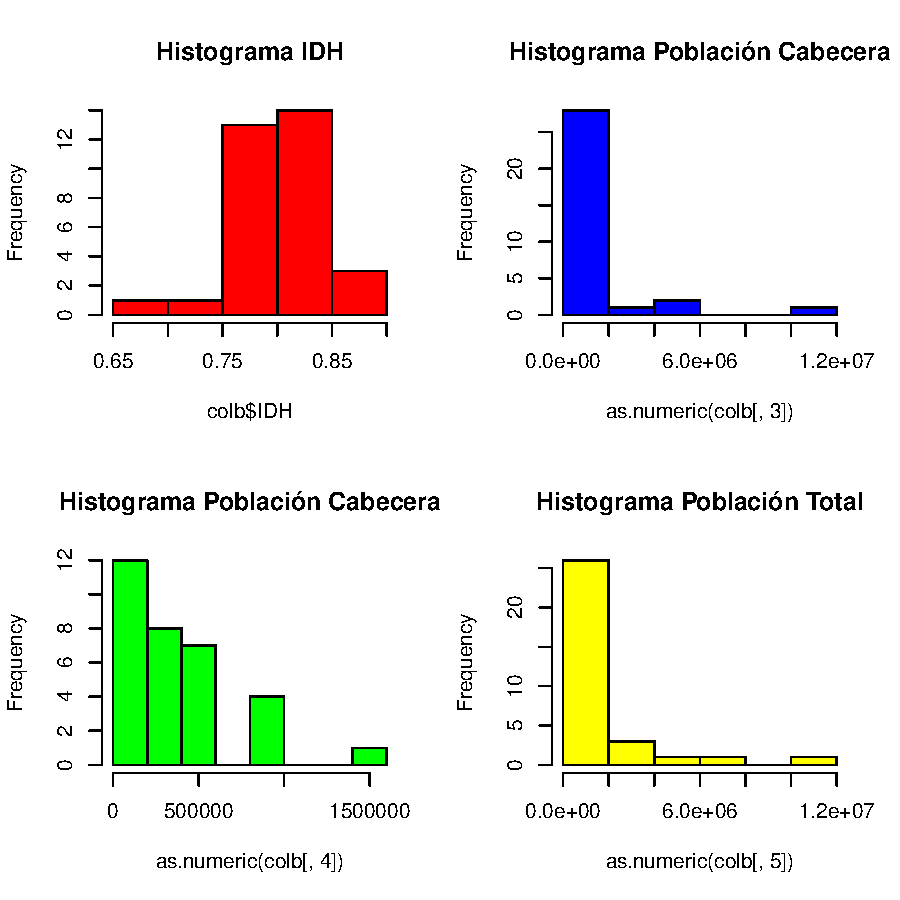
\includegraphics{EntregaFinal-barplots}
  
  
Dado el sesgo de las pobaciones,podriamos transformarla para que se acerque a la normalidad.

\begin{adjustbox}{width=9cm,height=3cm,clip,trim=1.5cm 0.5cm 0cm 1.5cm}
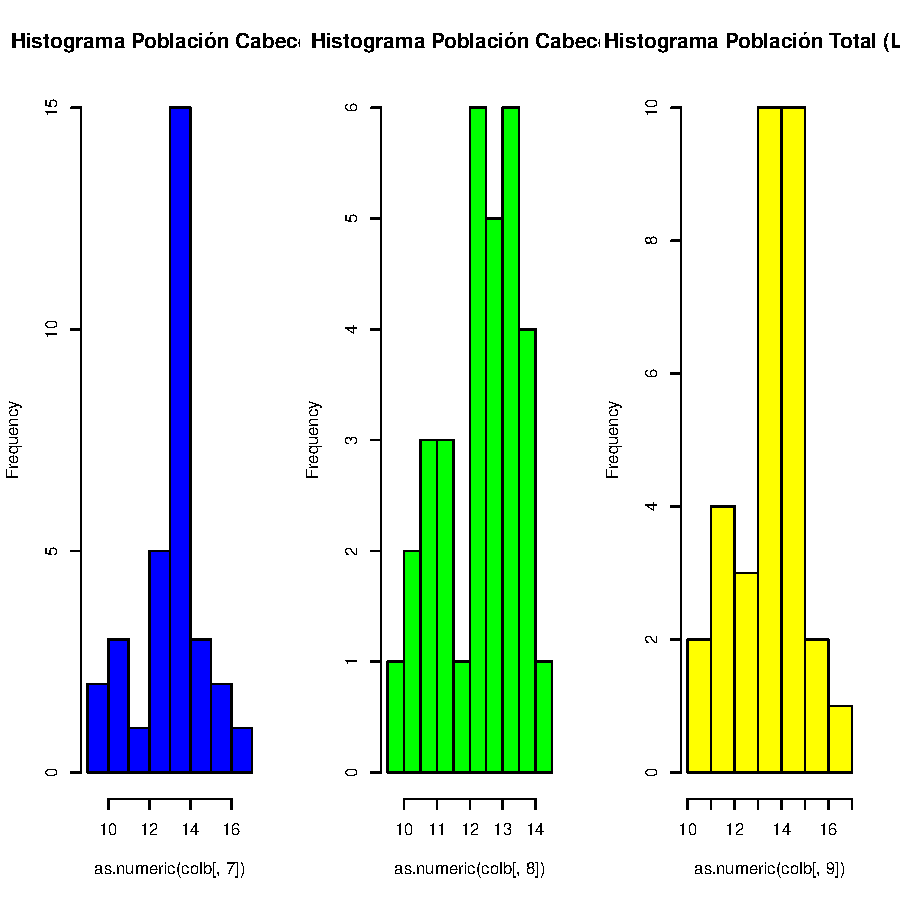
\includegraphics{EntregaFinal-barplots2}
\end{adjustbox}

 \caption{Distribución de Indicadores}
 \label{barplots}
 \end{figure}
 
 \clearpage

 \section{Exploración Bivariada}

En este trabajo estamos interesados en el impacto de la poblacion en el el IDH, veamos IDH con cada uno:
 
% Table created by stargazer v.5.2.2 by Marek Hlavac, Harvard University. E-mail: hlavac at fas.harvard.edu
% Date and time: vie., jun. 29, 2018 - 6:44:42 p. m.
\begin{table}[!htbp] \centering 
  \caption{Correlación de Democracia con las demás variables} 
  \label{corrDem} 
\begin{tabular}{@{\extracolsep{5pt}} ccc} 
\\[-1.8ex]\hline 
\hline \\[-1.8ex] 
cabeLog & restoLog & totaLog \\ 
\hline \\[-1.8ex] 
$0.487$ & $0.177$ & $0.424$ \\ 
\hline \\[-1.8ex] 
\end{tabular} 
\end{table} La correlación entre las variables independientes:

% Table created by stargazer v.5.2.2 by Marek Hlavac, Harvard University. E-mail: hlavac at fas.harvard.edu
% Date and time: vie., jun. 29, 2018 - 6:44:42 p. m.
\begin{table}[!htbp] \centering 
  \caption{Correlación de Democracia con las demás variables} 
  \label{corrTablex} 
\begin{tabular}{@{\extracolsep{5pt}} cccc} 
\\[-1.8ex]\hline 
\hline \\[-1.8ex] 
 & cabeLog & restoLog & totaLog \\ 
\hline \\[-1.8ex] 
cabeLog & 1 &  &  \\ 
restoLog & 0.84 & 1 &  \\ 
totaLog & 0.99 & 0.9 & 1 \\ 
\hline \\[-1.8ex] 
\end{tabular} 
\end{table} Visualmente:


Lo visto en la Tabla \ref{corrTableX} se refuerza claramente en la Figura \ref{corrPlotX}.

\begin{figure}[h]
\centering
\begin{adjustbox}{width=7cm,height=7cm,clip,trim=1.5cm 0.5cm 0cm 1.5cm}
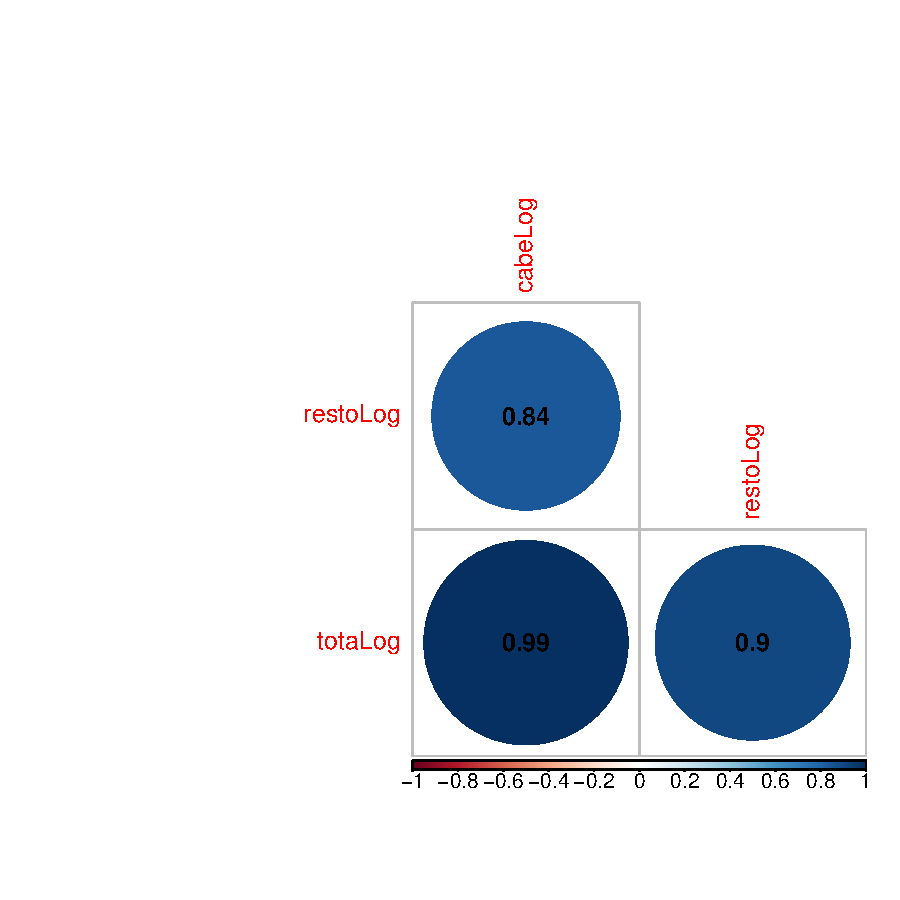
\includegraphics{EntregaFinal-corrPlotX}
\end{adjustbox}
\caption{correlación entre predictores}
\label{corrPlotX}
\end{figure}


\clearpage


 
\section{Modelos de Regresión}

Veamos los modelos propuestos. 
Primero sin poblacion resto, luego con esa:



Resultados
% Table created by stargazer v.5.2.2 by Marek Hlavac, Harvard University. E-mail: hlavac at fas.harvard.edu
% Date and time: vie., jun. 29, 2018 - 6:44:43 p. m.
\begin{table}[!htbp] \centering 
  \caption{Modelos de Regresión} 
  \label{regresiones} 
\begin{tabular}{@{\extracolsep{5pt}}lcc} 
\\[-1.8ex]\hline 
\hline \\[-1.8ex] 
 & \multicolumn{2}{c}{\textit{Dependent variable:}} \\ 
\cline{2-3} 
\\[-1.8ex] & \multicolumn{2}{c}{IDH} \\ 
\\[-1.8ex] & (1) & (2)\\ 
\hline \\[-1.8ex] 
 cabeLog & 0.013$^{***}$ & 0.066 \\ 
  & (0.004) & (0.046) \\ 
  & & \\ 
 restoLog &  & $-$0.016 \\ 
  &  & (0.020) \\ 
  & & \\ 
 totaLog &  & $-$0.051 \\ 
  &  & (0.064) \\ 
  & & \\ 
 Constant & 0.634$^{***}$ & 0.818$^{***}$ \\ 
  & (0.055) & (0.092) \\ 
  & & \\ 
\hline \\[-1.8ex] 
Observations & 32 & 32 \\ 
R$^{2}$ & 0.238 & 0.437 \\ 
Adjusted R$^{2}$ & 0.212 & 0.377 \\ 
Residual Std. Error & 0.037 (df = 30) & 0.033 (df = 28) \\ 
F Statistic & 9.347$^{***}$ (df = 1; 30) & 7.257$^{***}$ (df = 3; 28) \\ 
\hline 
\hline \\[-1.8ex] 
\textit{Note:}  & \multicolumn{2}{r}{$^{*}$p$<$0.1; $^{**}$p$<$0.05; $^{***}$p$<$0.01} \\ 
\end{tabular} 
\end{table} 
 \clearpage
 
\section{Exploración Espacial}

Calculemos conglomerados de regiones,usando toda la información de las tres variables.
Usaremos la tecnica de k-means propuesta por MacQueen.\cite{reynolds_clustering_2006}

Como acabamos de ver en la Tabla \ref{regresiones} en la página \pageref{regresiones}, si quisieras sintetizar la multidimensionalidad de nuestros indicadores, podrÃ?amos usar tres de las cuatro variables que tenemos (un par de las originales tiene demasiada correlación). 
 
%As�, propongo que calculemos conglomerados de pa�ses usando toda la información de tres de los indicadores. Como nuestras variables son ordinales utilizaremos un proceso de conglomeración donde las distancia serán calculadas usando la medida {\bf gower} propuestas en \cite{gower_general_1971}, y para los enlazamientos usaremos la técnica de {\bf medoides} según \cite{reynolds_clustering_2006}. Los tres conglomerados se muestran en la Figura \ref{clustmap}.
% 

% 
% 


% 
% 
% 
\begin{figure}[h]
\centering
%\begin{adjustbox}{width=11cm,height=8cm,clip,trim=1cm 2.5cm 0cm 2.5cm}
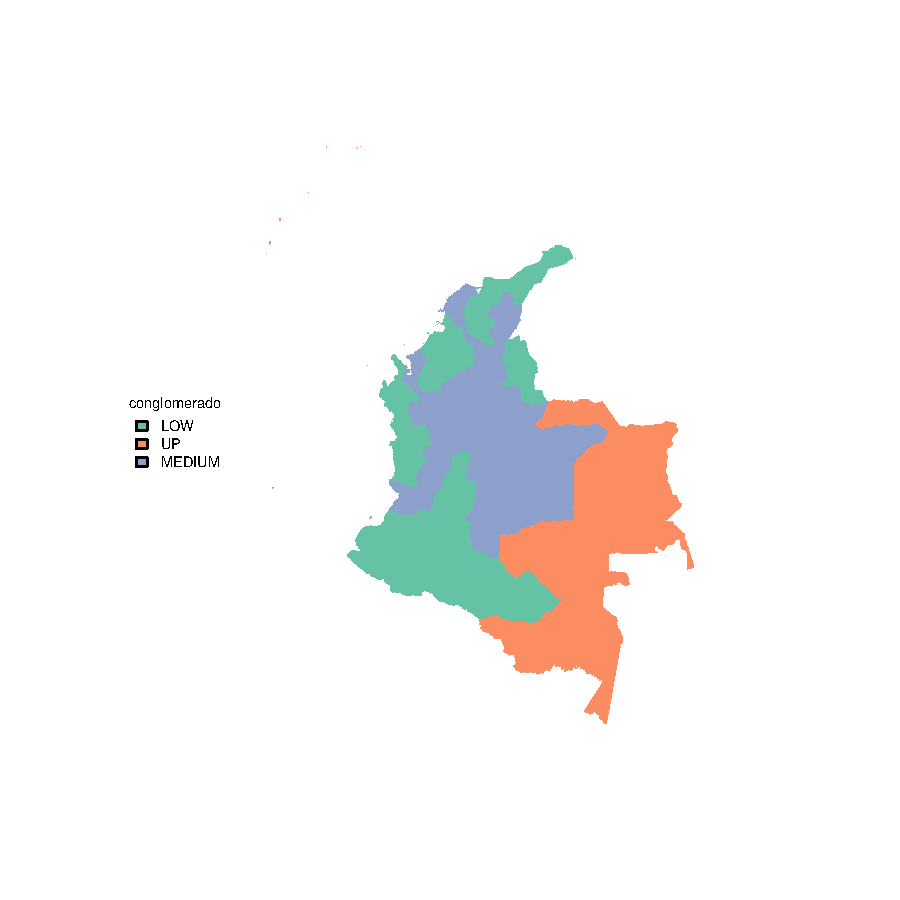
\includegraphics{EntregaFinal-plotMap1}

%\end{adjustbox}
\caption{Paises conglomerados segun sus indicadores sociopolÃ?ticos}\label{clustmap}
\end{figure}
% 
\bibliographystyle{abbrv}
\renewcommand{\refname}{Bibliography}
\bibliography{Colombia}

\end{document}
